% CVPR 2026 formatting; template files copied from the course intro submission.
\documentclass[10pt,twocolumn,letterpaper]{article}

\usepackage[pagenumbers]{cvpr}
\input{preamble}
\renewcommand{\ttdefault}{cmtt}

\usepackage{booktabs}
\usepackage{amsmath}
\usepackage{graphicx}

\definecolor{cvprblue}{rgb}{0.21,0.49,0.74}
\usepackage[pagebackref,breaklinks,colorlinks,allcolors=cvprblue]{hyperref}

\def\paperID{6.S058-Final}
\def\confName{CVPR}
\def\confYear{2026}

\title{Layered Typography-Aware Poster Generation\\
with Editable Text}

\author{Zhicheng Jiang\thanks{Equal contribution.}\\
Massachusetts Institute of Technology\\
{\tt\small jzc\_2007@mit.edu}
\and
Dingning Cao\footnotemark[1]\\
Massachusetts Institute of Technology\\
{\tt\small dcao2028@mit.edu}}

\begin{document}
\maketitle

\begin{abstract}
Text-to-image diffusion models can synthesize visually rich poster-like images, but they remain unreliable when the image must contain exact, editable, and well-composed text. We study this failure mode in text-heavy poster generation and propose a layered pipeline that separates visual synthesis from typography. Qwen-Image first generates a no-text background; a saliency- and contrast-aware layout module places structured text boxes; a learned typography-tool router selects fonts and display effects; and a deterministic renderer produces the final typography layer with strokes, shadows, gradients, local backing, and editable layout metadata. Because the background is fixed once generated, edits to typography never trigger regeneration --- and therefore never alter the underlying scene. On 24 poster-style prompts, our renderer achieves mean outside-text SSIM 0.997 and LPIPS 0.0049 across edited variants, while strong T2I baselines that re-prompt for new text routinely change the depicted subject (composition, identity, lighting). Our results suggest that treating typography as a structured layer is a practical path toward controllable text-heavy visual synthesis.
\end{abstract}

\section{Introduction}

Modern text-to-image (T2I) diffusion models such as latent diffusion models~\cite{rombach2022ldm}, Imagen~\cite{saharia2022imagen}, and DALL$\cdot$E-style systems~\cite{betker2023dalle3} can generate compelling images from natural-language prompts. Yet posters, advertisements, book covers, flyers, and social media graphics expose a persistent weakness: image generators often produce plausible visual compositions but fail to render precise text. Letters become pseudo-glyphs, words are misspelled, captions appear in the wrong place, and typography cannot be edited after generation. This is not only an aesthetic problem. Text-heavy visual synthesis requires exact symbolic content, spatial grounding, visual hierarchy, and downstream editability.

This problem matters because many practical uses of generative vision are not one-shot illustrations but editable design artifacts. A poster designer may want to keep a generated background while changing the event date, replacing the subtitle, or trying several brand messages. A small business owner may need a flyer whose headline is correct and whose visual scene remains stable after feedback. In these settings, the output is useful only if symbolic text can be controlled at the same level as visual appearance. The central research question of this project is therefore: can we obtain the visual richness of a modern T2I model while representing text as a structured layer that is exact, editable, and spatially grounded?

We address this setting through \emph{layered typography-aware poster generation}. Instead of asking a diffusion model to jointly invent imagery and rasterize text, we split the problem into background synthesis and structured typography. The model generates the visual scene without text; a layout planner selects candidate text regions; and a renderer writes exact strings as an editable text layer. The final output is both a raster poster and a JSON layout containing text, bounding boxes, colors, and roles. The key practical consequence is that the visual scene becomes a stable artifact: once a user accepts a background, subsequent text edits are cheap, deterministic, and structurally guaranteed to leave the scene unchanged. By contrast, re-prompting a T2I model with new text regenerates the entire image, so the scene drifts --- sometimes drastically, as when the depicted subject changes identity or composition between edits. This design is deliberately pragmatic: it uses diffusion models for the component where they are strongest and uses structured rendering for the component where exactness and stability matter most.

The project makes three contributions. First, we implement an end-to-end pipeline for poster generation with editable text layers. Second, we train compact modules: a layout ranker, a GenPoster-trained text-box prior, and a typography-tool router that chooses among multiple font/effect presets. Third, we evaluate with edit-preservation metrics, layout validity, style-router accuracy against a majority baseline, style diversity figures, and qualitative comparisons to direct T2I prompting. In the final version, we replace the early black-band typography with open-source display fonts and reusable effects such as neon glow, foil gradients, retro shadows, block shadows, letterpress, and stamp-like rendering. Although the approach is not an end-to-end text-rendering diffusion model, it produces a substantially more reliable system for the specific design task we target.

\section{Related Work}

\textbf{Text rendering in image generation.} Methods such as TextDiffuser~\cite{chen2023textdiffuser}, AnyText~\cite{tuo2024anytext}, and Glyph-ByT5~\cite{liu2024glyphbyt5} improve visual text rendering by injecting glyph- or character-level information into diffusion models. More recent text-capable backbones such as Qwen-Image render legible typography directly. These works show that explicit text supervision is important and that modern T2I models are no longer broken at text legibility. Two limitations remain. First, their outputs are raster images whose typography is not represented as a persistent editable layer: changing a single word requires re-running the generator. Second, regeneration does not preserve the surrounding scene --- re-prompting drifts composition, lighting, and even the identity of depicted subjects (\S\ref{sec:results}, Fig.~\ref{fig:qual}). Our system makes typography a first-class structured object and treats the background as a fixed asset, addressing both limitations simultaneously.

Our approach is complementary to these text-rendering models rather than a replacement for them. If the goal is a single image with visible words, an end-to-end text-aware diffusion model is attractive because the typography can be integrated into the lighting, perspective, and texture of the whole image. However, that same integration becomes a weakness for iterative design: the text cannot be selected as an object, reflowed, recolored, or edited without changing pixels outside the word. We therefore evaluate a different question: not whether a model can draw a word once, but whether a poster-generation system can preserve the scene while the text changes. This evaluation axis is closer to design-tool behavior than to ordinary image-generation fidelity.

\paragraph{Layout-aware generation.}
GLIGEN~\cite{li2023gligen}, ControlNet~\cite{zhang2023controlnet}, and LayoutGPT~\cite{feng2023layoutgpt} condition generation on spatial layouts or object boxes. These approaches provide more control than prompt-only generation, but the controlled elements are usually objects or semantic regions rather than typographic hierarchy. Our layout variables are text-specific: role, bounding box, color, and renderable string content.

These layout-control methods also differ in where the spatial constraint is applied. In GLIGEN or ControlNet-like systems, the layout typically guides the generative process itself, so the model still decides the final raster appearance of the controlled region. Our system applies spatial reasoning after background generation. This makes the layout layer simpler and less expressive, but easier to audit: every text box has explicit coordinates, every string is stored verbatim, and edits correspond to deterministic re-rendering rather than a new sampling process. The tradeoff is intentional for poster workflows where exactness and repeatability are more important than fully learned text texture.

\paragraph{Graphic and poster layout.}
PosterLayout~\cite{hsu2023posterlayout}, CGL-GAN~\cite{zhou2022cgl}, and AutoPoster~\cite{lin2023autoposter} study visual-textual presentation design and content-aware layout. Our work is closer to this line than to pure scene synthesis: the goal is a usable design artifact. However, we combine generated backgrounds, structured typographic rendering, and edit-preservation evaluation in a compact pipeline.

Prior poster-layout systems often assume a set of assets and text elements and focus on arranging them attractively. Our problem setting adds a generative background model and a strong direct T2I baseline, which creates a different set of failure modes. A direct T2I poster can look visually polished, but it may add extra words, hallucinate labels, or change the entire background when the user edits a single string. Our contribution is to connect poster-layout ideas with a modern image generator and to evaluate the system using background-preservation metrics rather than only text recognition or aesthetic quality.

\section{Method}

\begin{figure*}[t]
    \centering
    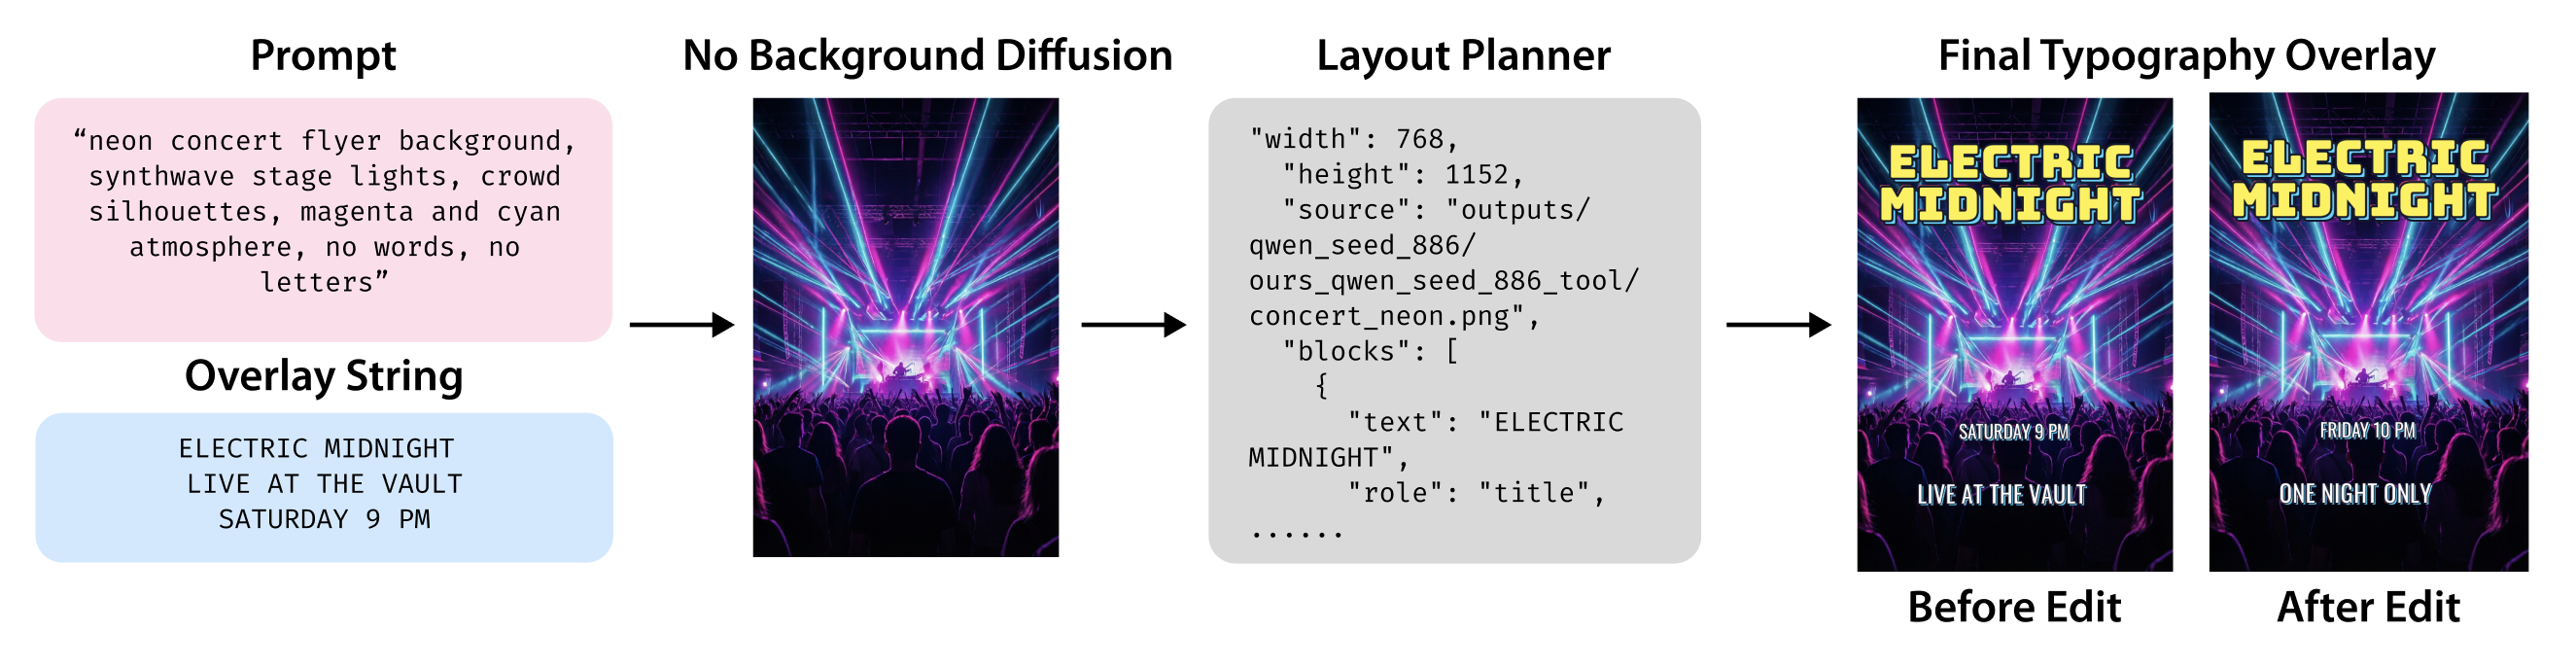
\includegraphics[width=0.96\linewidth]{figures/figure1_pipeline.png}
    \caption{\textbf{Pipeline.} We generate a no-text visual background, plan structured typography using saliency and contrast cues, render exact text deterministically, and preserve the layout as editable JSON metadata.}
    \label{fig:pipeline}
\end{figure*}

Given a prompt $p$ and text strings $\mathcal{T}=\{t_i\}_{i=1}^{n}$, our goal is to produce a poster image $I$ and a structured layout $L=\{(t_i, b_i, r_i, c_i)\}_{i=1}^{n}$, where $b_i$ is a bounding box, $r_i$ is a role such as title or metadata, and $c_i$ is a foreground color.

The method is designed to test one claim: for text-heavy visual synthesis, a layered representation can provide stronger editability than a single raster generated end-to-end. Each component therefore has a narrow role. Qwen-Image is responsible for the photographic or illustrative scene; the planner is responsible for text placement; the router is responsible for choosing an appropriate typography tool; and the renderer is responsible for exact symbolic content. This decomposition lets us isolate failures. If a background contains unwanted text, that is a background-generation failure. If a title overlaps an object, that is a layout failure. If an effect looks visually mismatched, that is a router/style failure. This separation makes the system easier to debug than a monolithic prompt-only baseline.

\paragraph{Background generation.}
For each poster prompt, we generate a background image using Qwen-Image. The background prompt describes only the visual scene and explicitly excludes text, letters, watermarks, signage, numbers, and logos. For comparison, we also generate a direct T2I baseline with the same base model, but its prompt asks the model to render the exact requested text inside the poster. Thus the comparison isolates two uses of the same image generator: direct rasterized poster generation versus no-text background synthesis followed by structured typography.

\paragraph{Candidate layout scoring.}
For title, subtitle, and metadata roles, we enumerate candidate boxes at several vertical anchors and horizontal offsets. Each candidate receives a hand-designed score:
\begin{equation}
s(b) = -E(b) - \lambda_o O(b) - \lambda_y |y_b - y_r| + \lambda_m M(b),
\end{equation}
where $E(b)$ is mean Sobel edge density inside the box, $O(b)$ penalizes overlap with previously selected text boxes, $y_b$ is the box center, $y_r$ is the role-specific preferred vertical location, and $M(b)$ is a margin bonus. Low edge density is a lightweight proxy for saliency and background clutter: placing text on low-edge regions tends to improve readability and avoids covering detailed visual content.

The candidate set is intentionally small enough to inspect but large enough to express common poster structures. For example, a title may be placed in a top, center, bottom, left-column, or full-width anchor depending on the style template, while metadata is biased toward margins or compact stacked regions. This differs from ordinary object layout, where the goal is often to place semantically meaningful objects. Here, the boxes are graphic-design affordances: they must leave the visual subject legible, create a typographic hierarchy, and reserve enough whitespace for display fonts. We therefore score boxes using both local image evidence and role-specific priors rather than only geometric overlap.

\paragraph{Learned layout ranker.}
We train a small MLP to predict the normalized candidate score. Each candidate is represented by 14 features: normalized $(x,y,w,h)$, normalized area, local edge mean and standard deviation, local luminance mean and standard deviation, normalized margin, distance to role-preferred vertical position, and a three-dimensional role one-hot vector. The network has two hidden layers with 64 and 32 units and is trained with mean-squared error. This ranker is not required for the deterministic fallback, but it provides a learned layout component and a natural bridge toward larger learned design models.

\paragraph{Typography-tool router.}
The first version of the system used a single high-contrast black-band style, which improved OCR but made outputs visually repetitive. We therefore add a tool registry with 19 typography presets: classic travel, cinematic, premium advertisement, Bauhaus, neon, literary, technology, sport, editorial serif, modern minimal, playful social, clean corporate, organic market, luxury fashion, retro pop, handmade marker, script invite, brutalist type, and space age. Each preset selects a layout template, font family, color palette, stroke width, shadow, tracking, backing mode, and display effect. The effects are implemented as deterministic rendering tools, not opaque online APIs: neon glow, foil or soft gradients, retro offset shadows, block shadows, letterpress, and stamp-like overlays. A small router predicts the preset from prompt keywords, category, text-length statistics, and weak design labels.

This router is deliberately weaker than a full aesthetic model. Its purpose is to choose a plausible tool family so that the renderer does not collapse to a single safe style. A travel poster should not use the same typography as a technology launch poster, and a literary cover should not look like a sports flyer. The weak labels are noisy, so we evaluate the router against a majority-class baseline and inspect the confusion matrix rather than treating the labels as ground truth taste judgments. In practice, the router gives the system enough stylistic range for the qualitative comparison while keeping all text editable.

\paragraph{Spatial refinement.}
The final system adds a template-aware spatial refinement pass. Candidate boxes are sized as a function of text length, clamped to safe margins, and augmented with poster-like anchor layouts. The scorer uses template-specific preferred vertical positions instead of one global title preference, and it penalizes both overlap and near-collisions between rendered text regions. This prevents bottom-title, editorial, and left-column styles from collapsing to the same layout and improves font-size hierarchy.

\paragraph{Poster-data layout prior.}
To move beyond hand-authored templates, we train on the full 102K-record GenPoster-100K annotation release~\cite{genposter100k}. Each record contains text-layer metadata including string content, bounding boxes, canvas size, font family, font size, and alignment. We construct positive examples from real text boxes and five random negatives per positive, then train a layout MLP with binary cross entropy. We also filter pathological skinny boxes and cluster per-style role boxes into reusable normalized priors. At rendering time, the planner combines these learned priors with saliency and contrast scoring, while enforcing a minimum title footprint so the learned prior does not collapse titles into small corner labels.

\paragraph{Typography rendering and editing.}
The selected text boxes are rendered with a deterministic FreeType-based renderer. The renderer fits font size to the box, wraps long strings, adds a high-contrast stroke, shadow, and translucent local backing band, and saves both the image and layout JSON. Editing is performed by changing the text strings and re-rendering only the typography layer on the same background.

The renderer stores every decision needed for later edits: the source background path, normalized box coordinates, role, font path, color, stroke, effect preset, alignment, and rendered string. This metadata is important because editability is not only the ability to draw correct text once. A useful design artifact must be re-opened, modified, and rendered again without reconstructing the prompt or sampling a new latent image. Our prototype exports raster posters rather than native design files, but the JSON layer is already close to a vector-tool representation: each text object has a stable identity and can be changed independently of the background.

\section{Experiments}

\paragraph{Dataset.}
We use 24 poster-style prompts spanning travel, film, product advertising, museum exhibitions, concerts, books, restaurants, technology events, fitness, education, beauty, music, food markets, architecture, transportation, games, fashion, photography, charity, board games, and cookbooks. Each prompt contains three text strings and an edited variant. For the final style/layout upgrade, we additionally train from GenPoster-100K metadata: 102,703 poster annotations, 102,699 with text layers, and 3,604,506 positive/negative layout examples.

\paragraph{Baselines.}
The main baseline is direct T2I generation with the same Qwen-Image model. The baseline prompt asks the model to produce the poster with the exact requested text. This is a strong practical baseline because it matches how users commonly attempt text-heavy image generation: one prompt requests both imagery and typography.

We use the same prompt set for background generation, direct T2I baselines, layered rendering, and edited variants. For Figure~\ref{fig:qual}, each group contains the no-text background, the direct Qwen baseline, and our final layered poster for the same prompt. For Figure~\ref{fig:style}, we deliberately use prompts disjoint from Figure~\ref{fig:qual} to show that the typography tools generalize beyond the examples used in the main qualitative comparison.

The comparison is therefore not between an old weak model and a new strong model. Both the background-only path and the direct baseline use Qwen-Image. The only difference is whether the model is asked to solve raster text generation directly or whether text is represented as a structured layer after image synthesis. This matters for interpreting the results: when the direct baseline misspells a word or changes the subject after an edit, the failure is not caused by using an obsolete backbone. It reflects a limitation of using a stochastic image generator as the only representation for a design object.

\paragraph{Metrics.}
We report rendered text exactness, layout validity, a contrast proxy, style-router accuracy, and edit background preservation. Layout validity is the fraction of boxes that are in-bounds and non-overlapping. Edit preservation is measured across the 24 prompt/edit pairs by masking the union of before- and after-edit text boxes, then computing SSIM~\cite{wang2004ssim} and LPIPS outside the masked regions. We treat OCR as a diagnostic rather than a primary metric because Tesseract~\cite{smith2007tesseract} is sensitive to local installation, stylized display fonts, and textured poster backgrounds.

The mask-based edit metric is the most important quantitative measurement in the report. Without masking, changing the title would trivially lower image similarity because the text pixels are supposed to change. With the union mask, the metric asks a more useful question: after the requested typography edit, did anything outside the editable text layer change? A score near perfect is expected for a deterministic renderer, but reporting it is still valuable because it states the guarantee in image-space terms and makes the contrast with re-prompted T2I outputs explicit.

\paragraph{Implementation details and reproducibility.}
The Qwen generations use the FP8 Qwen-Image checkpoint on an RTX 5090, with 20 diffusion steps, true-CFG scale 4.0, and 768-by-1152 poster canvases. We store every generated background, direct baseline, final rendered poster, edit pair, and layout JSON in the project workspace. The main paper figures are reproducible from the committed scripts: \texttt{generate\_images.py} creates no-text backgrounds and direct T2I baselines, \texttt{render\_posters.py} renders the structured text layer, \texttt{create\_edits.py} creates edited variants, \texttt{evaluate.py} computes layout and edit-preservation metrics, and the figure scripts assemble the grids. We include the prompt files, style maps, generated figures, and summary metrics in the repository so that the reported comparisons can be inspected without rerunning Qwen.

The layout ranker is trained on 1,248 candidate boxes generated from the diagnostic prompt set. The GenPoster layout prior is trained from 102,703 annotations and 3,604,506 positive/negative box examples. The typography-tool router is trained on 99,996 weakly labeled style examples for 120 epochs across hidden widths and seeds, and we report the best validation accuracy. The router is evaluated against a majority-class baseline to avoid overstating performance on imbalanced weak labels.

\begin{table}[t]
    \centering
    \caption{Main quantitative diagnostics over 24 prompts and edited variants. Edit preservation is measured outside the union of before/after text-box masks.}
    \label{tab:main}
    \begin{tabular}{lc}
        \toprule
        Metric & Value \\
        \midrule
        Layout validity\footnotemark & 1.000 \\
        Contrast proxy & 0.526 \\
        Edit outside-mask SSIM $\uparrow$ & 0.997 \\
        Edit outside-mask LPIPS $\downarrow$ & 0.0049 \\
        Edited prompt pairs & 24 \\
        \bottomrule
    \end{tabular}
\end{table}
\footnotetext{Layout validity is enforced by the planner; the reported value indicates that the planner produced a valid in-bounds non-overlapping configuration on every prompt in the test set, i.e.\ the search never failed to find a feasible layout.}

\begin{table}[t]
    \centering
    \caption{Learned layout and typography-tool priors. The router uses weak pseudo-labels, so its accuracy measures tool-selection consistency rather than human aesthetic preference.}
    \label{tab:style}
    \begin{tabular}{lc}
        \toprule
        Quantity & Value \\
        \midrule
        Poster annotations for layout & 102,703 \\
        Layout examples & 3,604,506 \\
        Layout validation accuracy & 0.975 \\
        Router training examples & 99,996 \\
        Typography-tool presets & 19 \\
        Router validation accuracy & 0.789 \\
        Majority-class baseline & 0.398 \\
        \bottomrule
    \end{tabular}
\end{table}

\begin{table}[t]
    \centering
    \caption{Layout ranker training summary. The validation correlation indicates that the lightweight MLP learns the candidate-box scoring objective.}
    \label{tab:training}
    \begin{tabular}{lc}
        \toprule
        Quantity & Value \\
        \midrule
        Candidate boxes & 1248 \\
        Train / validation & 998 / 250 \\
        Feature dimension & 14 \\
        Epochs & 450 \\
        Final validation MSE & 0.200 \\
        Final validation correlation & 0.887 \\
        \bottomrule
    \end{tabular}
\end{table}

\section{Results}
\label{sec:results}

\begin{figure*}[t]
    \centering
    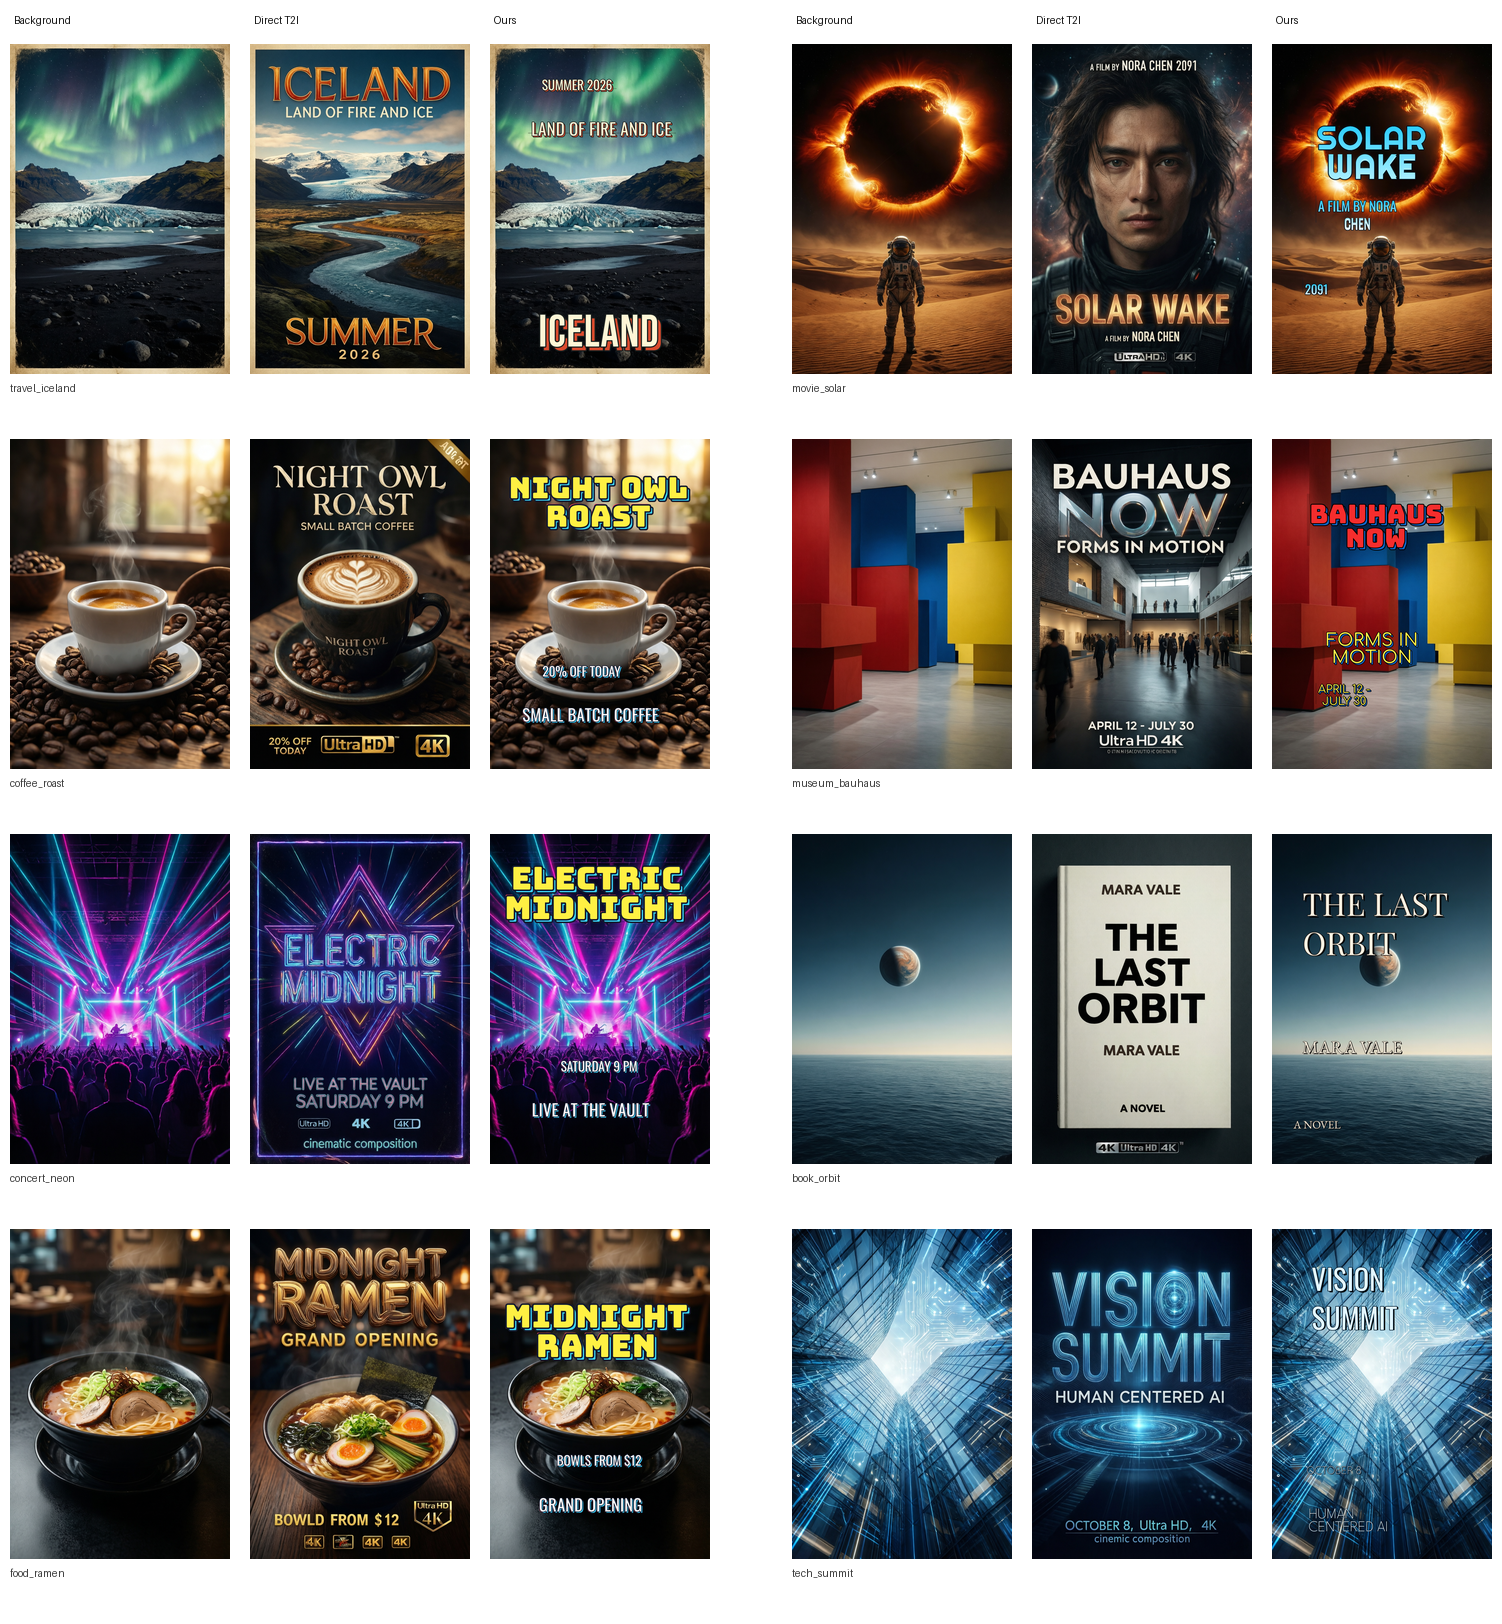
\includegraphics[width=0.96\linewidth,height=0.72\textheight,keepaspectratio]{figures/qualitative_grid.png}
    \caption{\textbf{Qualitative comparison.} Each group shows a no-text Qwen background, a direct Qwen T2I poster baseline, and our layered result. Direct T2I baselines are visually strong but often introduce extra text, pseudo-text, or non-editable raster typography. Our method uses generated backgrounds but renders the requested typography as a structured layer.}
    \label{fig:qual}
\end{figure*}

\begin{figure*}[t]
    \centering
    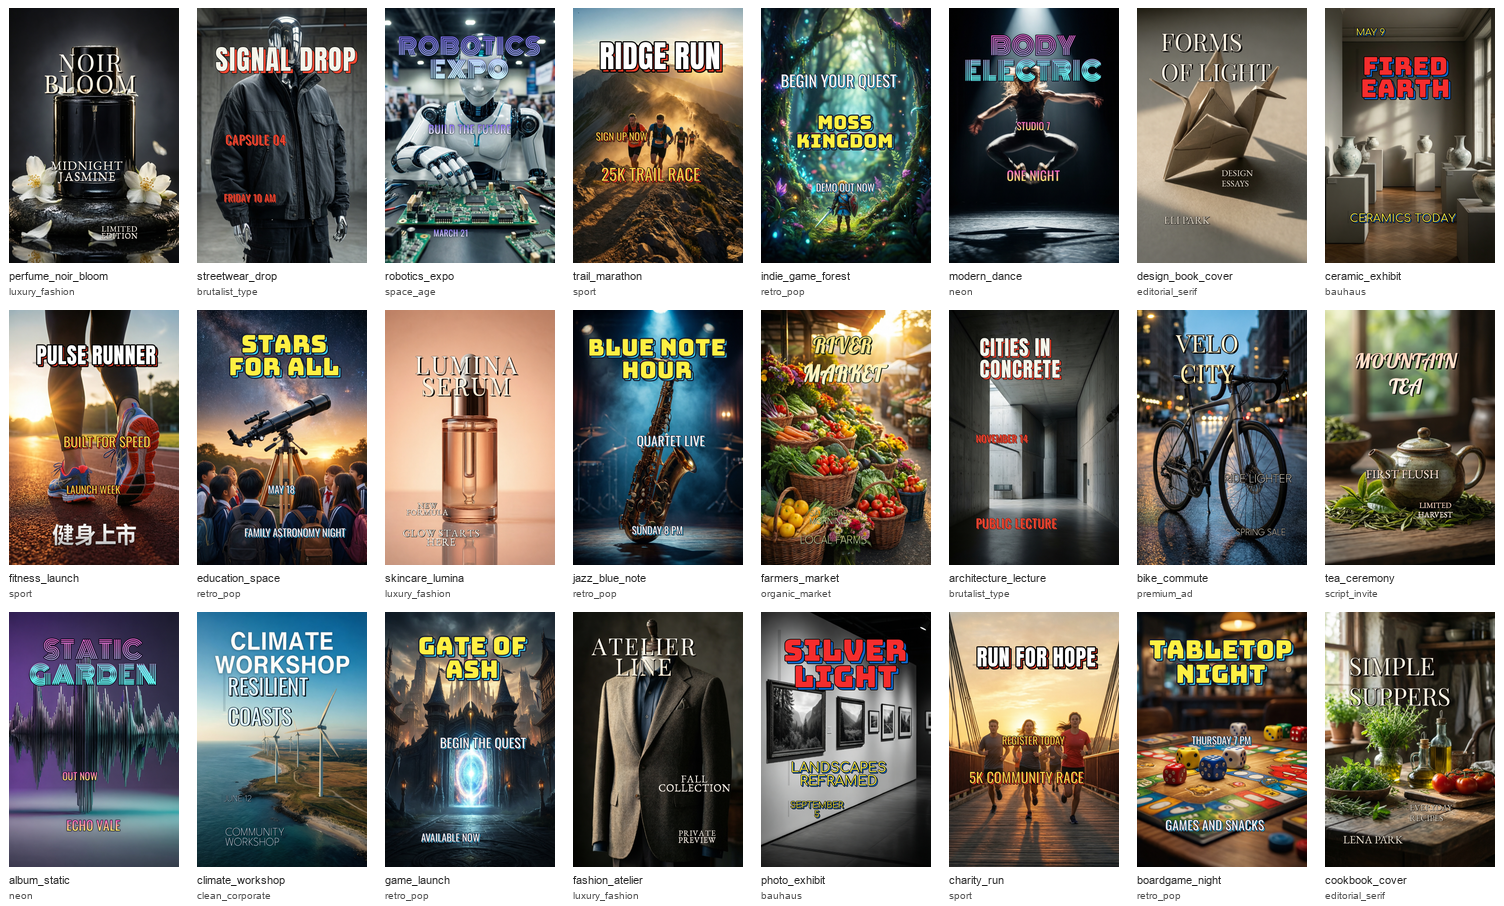
\includegraphics[width=0.98\linewidth,height=0.76\textheight,keepaspectratio]{figures/style_grid_mixed_no_overlap.png}
    \caption{\textbf{Typography-tool routing.} This gallery uses prompts disjoint from Fig.~\ref{fig:qual}. The learned router selects different font families, layout templates, and display effects for different poster categories, avoiding the single-style black-band appearance of the first prototype.}
    \label{fig:style}
\end{figure*}

Our main empirical claim is edit preservation. Table~\ref{tab:main} reports mean SSIM and LPIPS outside the union of before- and after-edit text-box masks across 24 prompt/edit pairs. The outside-mask SSIM is 0.997 and LPIPS is 0.0049, showing that changing a title, subtitle, date, or callout leaves the generated background effectively unchanged. Because the final text is rendered from structured strings, rendered text exactness is 1.000 by construction; we therefore treat exactness as a system property rather than the central quantitative result.

The practical importance of this number is that re-prompting a strong T2I model with new text does not, in general, preserve the depicted scene. In our 24-prompt comparison, the direct Qwen baseline frequently regenerates non-typographic content when only the strings change: subjects shift pose, lighting changes, and in several cases the depicted entity itself is replaced. In the Solar Wake panel of Fig.~\ref{fig:qual}, for example, the direct baseline introduces a human face that is absent from our no-text background; re-prompting with a different subtitle would yield yet another face. This is not a failure of Qwen --- it is a structural property of any pipeline that re-runs the generator per edit. Our pipeline never re-runs the generator after the background is accepted, so the scene is identical across edits up to typography rasterization. The SSIM and LPIPS values reflect this guarantee empirically; the qualitative pairs in Fig.~\ref{fig:edit} demonstrate it visually.

The second claim is that the poster-data layout prior is useful for practical typography placement. The GenPoster-trained layout model reaches 0.975 validation accuracy over real and negative text boxes, and the planner produced a valid in-bounds non-overlapping configuration for every prompt in the 24-prompt set, i.e.\ the search never failed to find a feasible layout under our spatial constraints. The direct T2I baseline in Figure~\ref{fig:qual} often creates plausible poster-like raster text, but it also adds unwanted labels, small glyphs, or ``4K''-style artifacts and provides no editable layout.

The third claim is style diversity through tool routing. The router reaches 0.789 validation accuracy against weak GenPoster-derived labels, compared with a 0.398 majority-class baseline. Figure~\ref{fig:style} shows the resulting visual variety: the system routes prompts to display fonts and effects such as condensed travel type, neon/retro shadows, editorial serif, Bauhaus geometry, luxury serif, and sport block lettering.

The qualitative grids are meant to support these three empirical claims rather than serve as isolated cherry-picked images. Figure~\ref{fig:qual} emphasizes the controlled comparison: for each prompt, the left image is the same kind of no-text Qwen background used by our system, the middle image is the direct Qwen poster baseline, and the right image is the layered output. This makes it possible to see both what Qwen contributes and what the typography layer changes. Figure~\ref{fig:style} then removes prompt overlap with Fig.~\ref{fig:qual} and uses a broader set of categories to stress-test the router's stylistic range. Figure~\ref{fig:edit} focuses on the edit operation itself: the visual background stays fixed while only the requested text layer changes.

The qualitative results also reveal the main tradeoff of the layered approach. Our outputs are more controllable and more editable, but the typography is intentionally rendered as a design layer rather than hallucinated as part of the scene. This means our text is exact and stable, but it may not inherit all subtle physical effects that an end-to-end generator could synthesize, such as text painted onto a curved object or embossed into a material. For posters, advertisements, and event flyers, this is usually acceptable because professional tools also treat typography as a layer. For scenes where text must be physically integrated into objects, a text-aware diffusion model or image-editing model could be used as a later refinement stage.

\begin{figure*}[t]
    \centering
    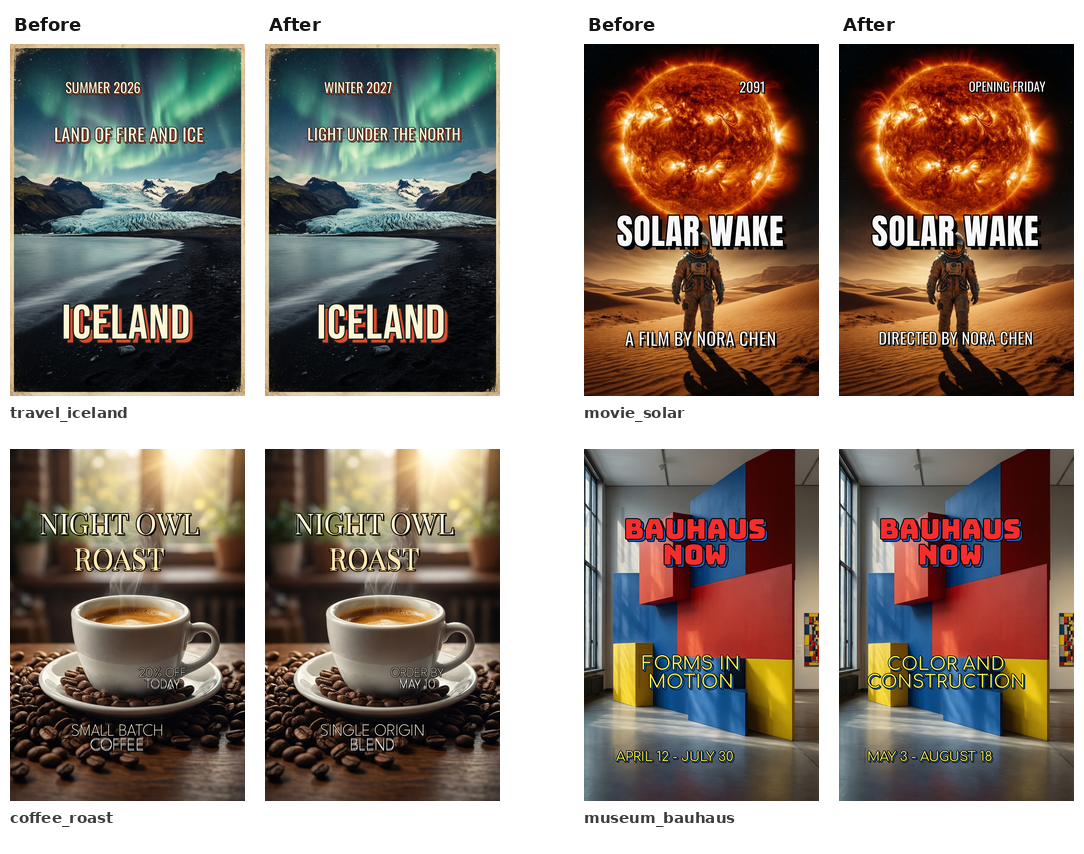
\includegraphics[width=0.88\linewidth,height=0.72\textheight,keepaspectratio]{figures/edit_examples.png}
    \caption{\textbf{Text editing.} Since text is a structured layer, changing a subtitle, date, or callout does not require regenerating the background.}
    \label{fig:edit}
\end{figure*}

\section{Ablations}

We compare the full system to two earlier variants on the original ten-prompt diagnostic subset: removing the edge-density saliency term and disabling high-contrast color selection. Table~\ref{tab:ablation} summarizes the diagnostic OCR results from the environment where Tesseract was available. The no-contrast variant reduces OCR exact match from 0.667 to 0.600 and lowers the contrast proxy from 0.676 to 0.602. The no-saliency variant places text over slightly higher-edge regions on average, increasing mean text-region edge density from 0.316 to 0.328. Although its OCR exact match is slightly higher on this small sample, its placements are often less compositionally balanced and more likely to interfere with salient content.

These ablations explain why the final system keeps both visual and structural constraints. Contrast-aware rendering improves local readability, but contrast alone can produce heavy bands that dominate the poster. Saliency-aware placement avoids busy background regions, but placement alone cannot guarantee legibility if the chosen font color is too close to the underlying image. The final renderer combines both signals with style-specific templates: saliency and learned priors decide where text can go, while the style preset decides how it should look once placed.

\begin{table}[t]
    \centering
    \caption{Ablations. The contrast-aware renderer improves text readability, while saliency-aware layout reduces background clutter under text boxes.}
    \label{tab:ablation}
    \resizebox{\linewidth}{!}{
    \begin{tabular}{lcccc}
        \toprule
        Variant & OCR Exact & Word Recall & Contrast & Edge Density \\
        \midrule
        Full & 0.667 & 0.854 & 0.676 & 0.316 \\
        No saliency & 0.700 & 0.843 & 0.677 & 0.328 \\
        No contrast & 0.600 & 0.816 & 0.602 & 0.316 \\
        \bottomrule
    \end{tabular}}
\end{table}

\begin{figure}[t]
    \centering
    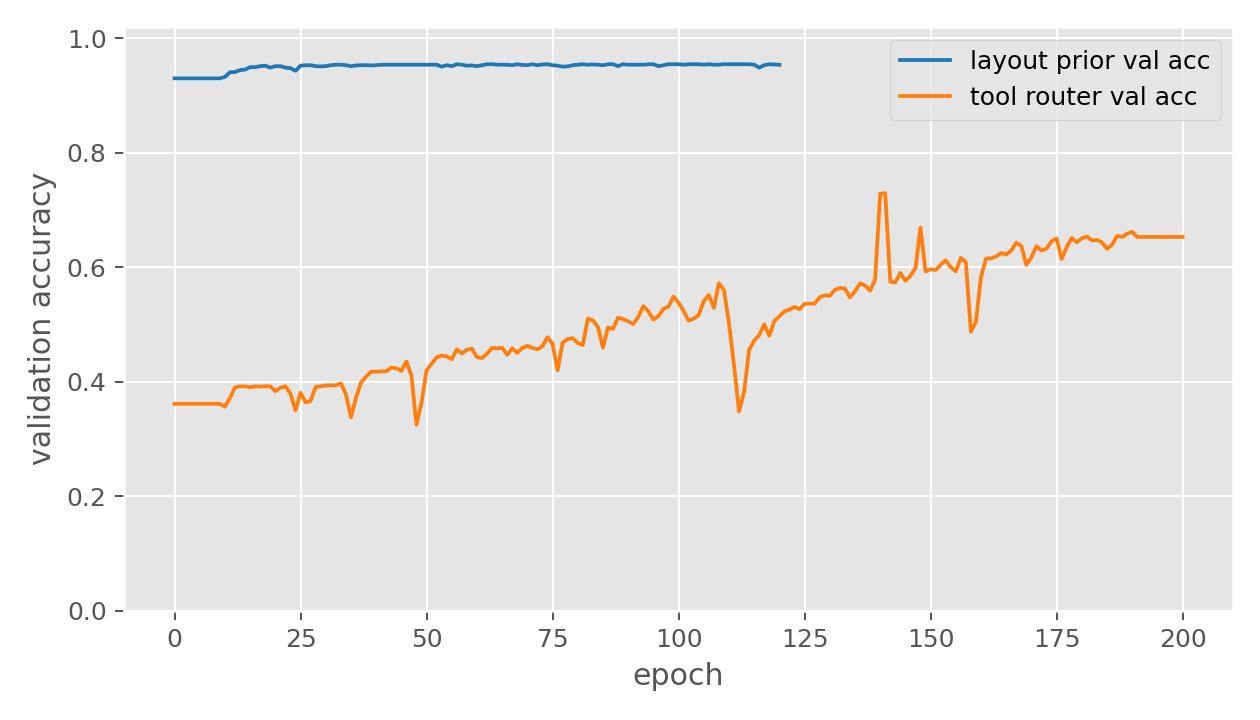
\includegraphics[width=0.98\linewidth]{figures/spatial_training_curve.png}
    \caption{\textbf{Training curves} for the GenPoster layout prior and the typography-tool router. The layout prior converges quickly to high validation accuracy; the router accuracy is bounded by the noise of weak GenPoster-derived style labels.}
    \label{fig:training}
\end{figure}

\section{Supplementary Diagnostics}

\begin{figure}[t]
    \centering
    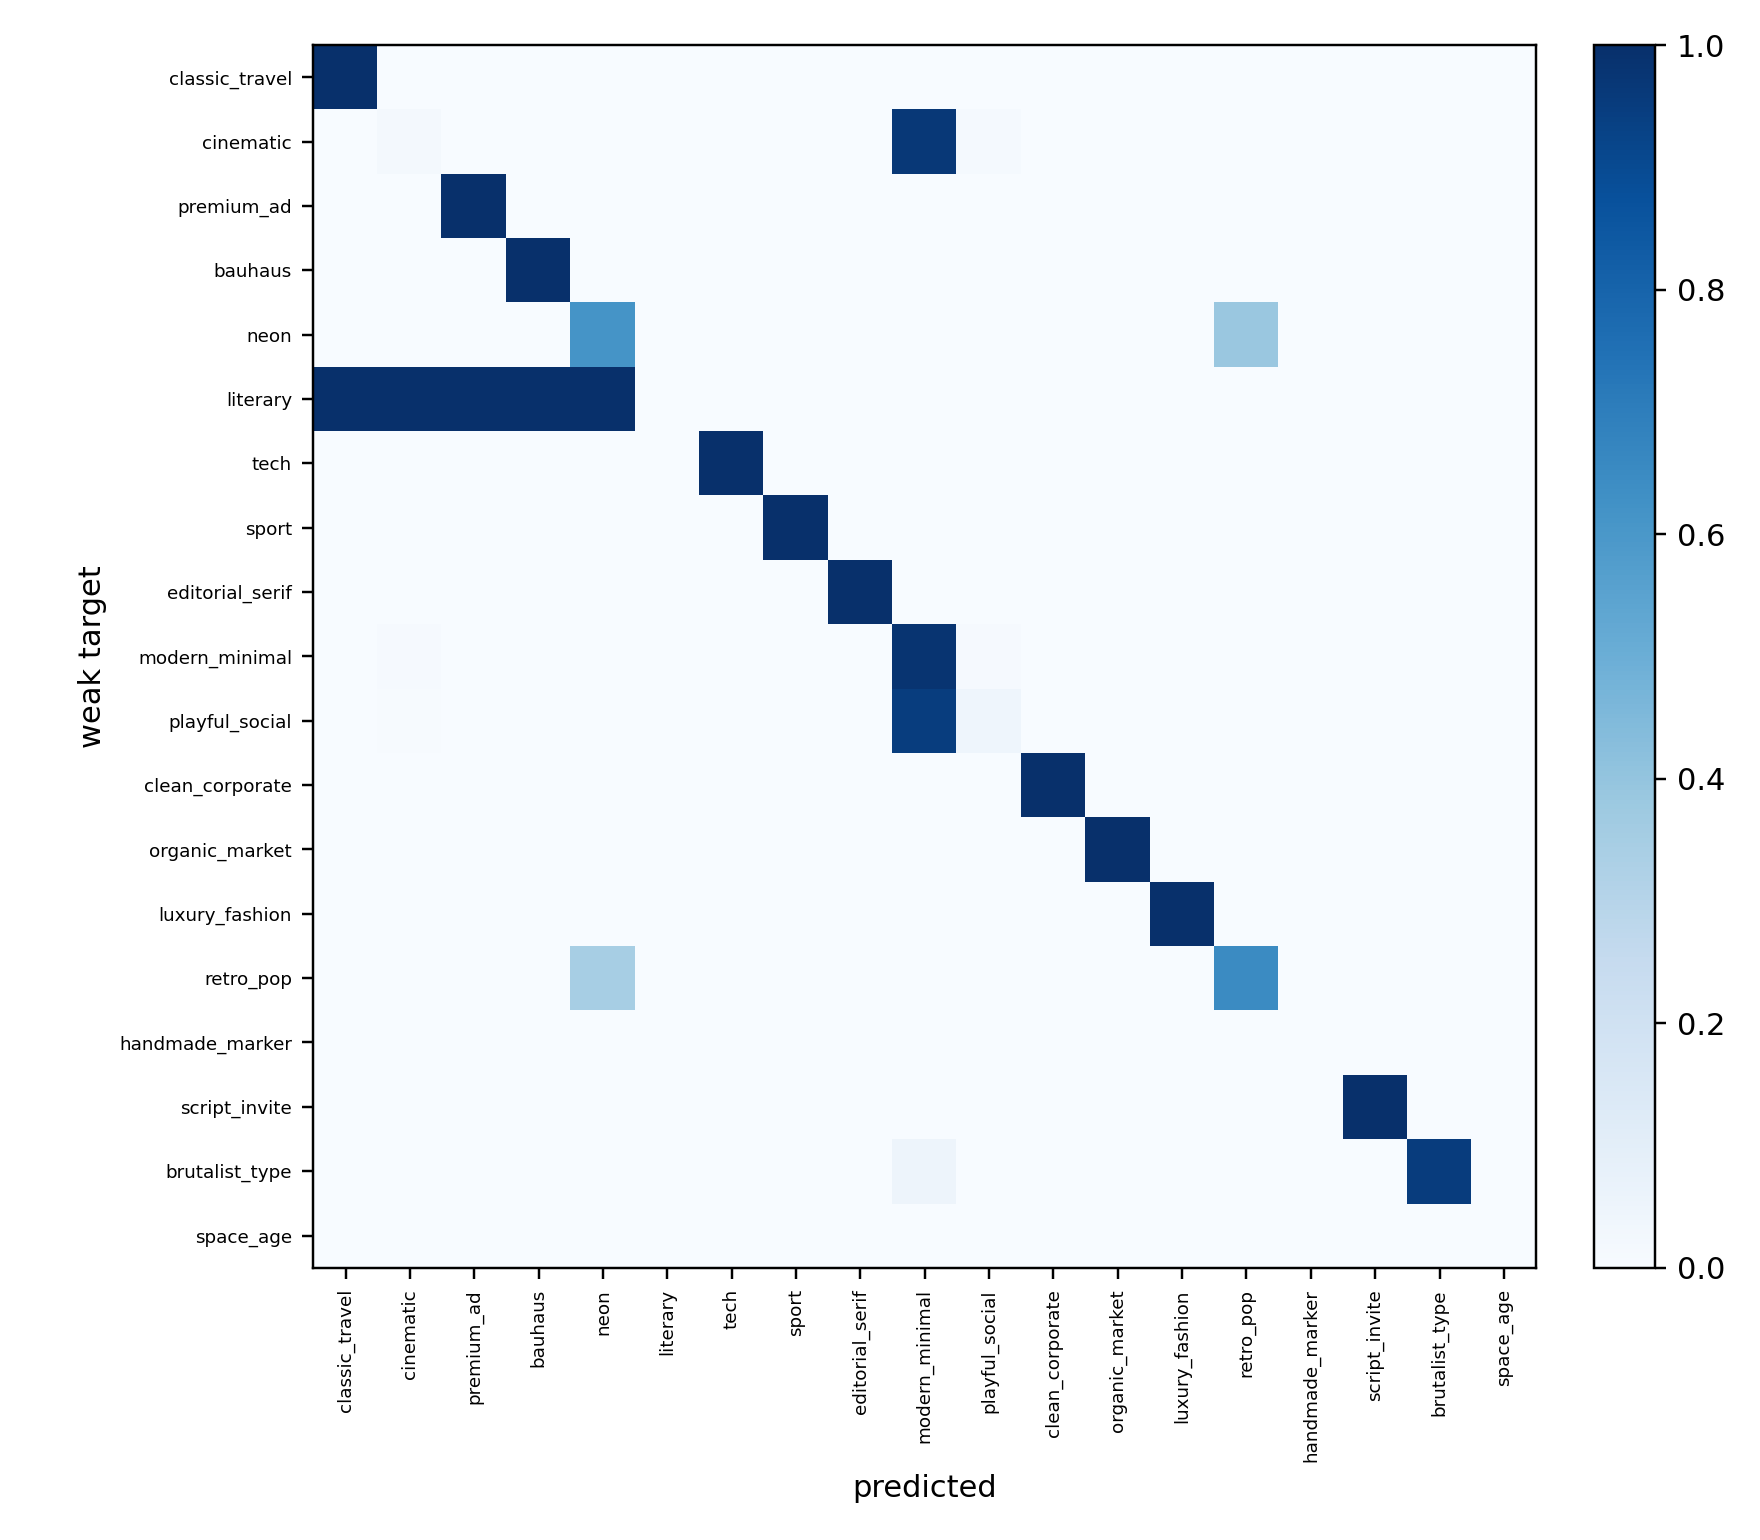
\includegraphics[width=0.98\linewidth]{figures/tool_router_confusion.png}
    \caption{\textbf{Typography-tool router confusion matrix.} Rows are weak GenPoster-derived target styles and columns are predicted tool presets. The router is not a human aesthetic judge; it is a compact controller that maps prompt/design cues to reusable typography tools.}
    \label{fig:confusion}
\end{figure}

Figure~\ref{fig:confusion} gives the supplementary confusion matrix requested for the tool router. The main confusions reflect the weak-label construction: modern minimal, cinematic, playful social, and retro pop are broad buckets, while rare classes such as space age and brutalist type have very limited support. This supports our interpretation of the router as a diversity controller rather than a definitive style classifier.

The confusion matrix also helps explain why style accuracy is not the headline result. Some mistakes are semantically acceptable: a clean corporate flyer and a modern minimal flyer can share fonts, spacing, and muted palettes, while a cinematic poster and a luxury advertisement can both use high-contrast serif typography. Other mistakes are more visible, such as routing a playful market prompt to a rigid technology preset. In the current system, these errors affect aesthetics but not text correctness or edit preservation. This separation is useful because a user can re-render the same background with another preset without paying the cost of image generation.

\section{Ethical and Societal Considerations}

The system is intended for controllable poster and flyer generation, but it inherits several risks from generative image models. First, Qwen-Image may reproduce dataset biases in how it depicts people, places, products, and cultural styles. If the system is used for real advertising or public communication, users should audit generated backgrounds for stereotypes, misleading visual claims, or inappropriate cultural associations before accepting them as fixed assets. Second, exact editable text makes it easier to generate polished misinformation, counterfeit event posters, or deceptive product advertisements. Our pipeline does not solve misuse by itself, but the structured layout JSON provides a useful mitigation path: generated outputs can retain metadata about the requested strings, edit history, and rendering pipeline. Such metadata could support provenance tools or human review in deployment.

Third, the distinction between direct T2I text and layered text has accessibility implications. Because our text layer is structured, it can be exported with machine-readable strings and bounding boxes, which is preferable to text that exists only as pixels. This could make generated posters easier to adapt to screen readers, alternate layouts, or localization workflows. However, the current prototype does not yet export accessible HTML or PDF text layers; it stores JSON metadata and raster images. A production version should preserve text semantics through the final publishing format.

Finally, our evaluation intentionally downweights OCR as the central metric because stylized text can be visually readable to humans while failing an OCR engine. This choice avoids optimizing solely for machine recognition, but it also means our system should not be treated as automatically accessible or correct. Human inspection remains necessary for safety-critical posters, public instructions, and medical, political, or financial communications.

\section{Limitations}

Our method is a layered design system rather than a fully end-to-end diffusion model. It does not learn kerning, curved text, custom font generation, or complex multi-line hierarchy at the level of a professional design tool. The Qwen background generator can occasionally insert unwanted text even when the background prompt forbids it, so strict no-text background generation remains imperfect. We note that this caveat applies only to the initial background; once the background is accepted, the no-regeneration property holds for all subsequent edits regardless of imperfections in the seed image. The GenPoster style labels are weakly supervised from metadata and prompt heuristics rather than human aesthetic preferences, so the router is best understood as a diversity controller rather than a definitive design critic. OCR is also an imperfect proxy: Tesseract can miss words that are visually correct to a human reader, especially when text is small, stylized, or placed on textured backgrounds. Still, for time-limited text-heavy design tasks, the layered approach offers a reliable tradeoff between visual quality, exact text, style control, and editability.

There are also limits in the experimental evidence. The 24-prompt set is broad enough to test the intended poster workflow, but it is not a large benchmark. We do not run a human preference study, so claims about visual quality are qualitative and supported by examples rather than statistically measured taste. The direct T2I baseline is strong and fair in the sense that it uses the same Qwen backbone, but prompt engineering could produce different individual images. For that reason, we avoid claiming that layered rendering is universally more beautiful than direct generation. The narrower claim is that it is more reliable for exact, editable text and background-preserving edits.

Future work could connect the layered renderer to a true vector graphics backend, so that the output remains editable in standard design tools rather than only through our JSON format. Another direction is learned aesthetic ranking: the current router predicts weak style labels, but it does not know whether a human designer would prefer one layout over another. A small human preference dataset could train a reranker over multiple layout/style candidates. Finally, the background generator could be constrained with stronger no-text controls or post-generation text removal so that the initial image is cleaner before typography is added. A stronger hybrid system could also pass the layered result through a localized image-editing model to integrate shadows or material effects while freezing pixels outside a narrow text neighborhood.

\section{Conclusion}

We presented a typography-aware poster generation pipeline that separates background synthesis from editable text rendering. The approach supports stable edits without background regeneration and avoids asking a T2I model to rasterize exact, editable typography. A lightweight trained layout ranker, a GenPoster layout prior, and a typography-tool router provide learned control over placement and visual style, while ablations show how saliency and contrast cues contribute to practical typography placement. More broadly, the project suggests that text-heavy visual synthesis should expose structured, editable layers rather than treating all visual content as a single raster generated from a prompt.

\section{Use of Generative AI}

Generative AI tools were used to help draft and revise prose, organize the CVPR-style report structure, and debug code/LaTeX. The experiments, scripts, generated figures, metrics, and final edits were run and verified in the project workspace.

\section{Team Contributions}

Zhicheng Jiang was responsible for the algorithmic design and implementation, running the training and generation experiments, writing the Method section, and producing the quantitative/data figures used in the report. Dingning Cao was responsible for dataset work, writing the Related Work section, and producing the other report figures. Both authors discussed the problem framing, interpreted results, reviewed the final report, and approved the submitted version.

{
    \small
    \bibliographystyle{ieeenat_fullname}
    \bibliography{main}
}

\end{document}
